% !TEX program = xelatex
\documentclass[11pt]{article}
\usepackage[margin=1in]{geometry}
\usepackage{nopageno} % no page numbers
\usepackage{setspace} \singlespacing

\usepackage{graphicx}
\graphicspath{ {./graphics/} }
\usepackage[dvipsnames]{xcolor}
\definecolor{CrispBlue}{HTML}{0176AE}

\usepackage{fontspec}
\usepackage{tcolorbox}
\usepackage{etoolbox}
\BeforeBeginEnvironment{verbatim*}{\begin{tcolorbox}[colback=CrispBlue!5!white,colframe=CrispBlue!75!black]}%
\AfterEndEnvironment{verbatim*}{\end{tcolorbox}}%

\usepackage{hyperref}
\hypersetup{
    colorlinks,
    citecolor=black,
    filecolor=black,
    linkcolor=black,
    urlcolor=black
}

\renewcommand{\footnotesize}{\fontsize{8pt}{10pt}\selectfont}


\usepackage[labelfont={small,sc,bf},textfont={small,sc,bf}]{caption}
\setlength{\parindent}{18pt}
% \setlength{\parskip}{1em}

\usepackage{tocloft}
\renewcommand{\cftpartleader}{\cftdotfill{\cftdotsep}}
\renewcommand{\cftsecleader}{\cftdotfill{\cftdotsep}}

\usepackage[shortlabels]{enumitem}

\usepackage{lastpage}
\usepackage{fancyhdr}
\pagestyle{fancy}
\fancyhf{}
\renewcommand{\headrulewidth}{0pt}
\rfoot{Page \thepage\ of \pageref*{LastPage}}

\usepackage{amsmath,amsfonts,amssymb}
\usepackage{bm}
\usepackage{mathtools}

\renewcommand{\listfigurename}{List of Figures}

\begin{document}
\setmainfont{Times New Roman}
\setsansfont{Times New Roman}
\setmonofont{Times New Roman}
\renewcommand{\familydefault}{\sfdefault}

\hypersetup{
    linkcolor=CrispBlue,
    urlcolor=CrispBlue,
    breaklinks=true
}

\noindent David Kirby\\
ECE 590: Graduate Seminar\\
Seminar 12 -- 15 April 2022 -- Dr. Weiwen Jiang\\
Towards Quantum AI Democratization\\

Professor Weiwen Jiang is an assistant professor at George Mason University. Before that he was a post-doc at the University of Notre Dame. He built the first co-design framework called quantum flow to demonstrate the quantum advantage in designing neural network onto a quantum computer, which was published in Nature Communications. This talk was about the topic of quantum AI democratization and their philosophy that they want to build a quantum neural network design state.

Before he introduced the details of the quantum AI, he wanted to go back to classic computing and the classical AI democratization. Classical AI democratization is a concept proposed by Fei-Fei Li from Google in 2017. The key idea is that they want to enable everyone to leverage AI to change our daily lives -- the keyword being \textit{everyone} gets the benefits, not just a few people. Dr. Jiang then presents some applications including medical AI scenarios. He shows that AI can indeed be beneficial for medical staff. There were two scenarios presented, the first being AR/VR in surgery and the second was medical diagnosis. AI can be used to perform real-time MRI segmentation and COVID CT segmentation. While it is obvious that AI can be beneficial, the question is can we expect doctors to design the neural networks that are necessary for the machine learning by themselves -- the answer of course was no. They do not have the strong background on how to design the algorithm. This is the main motivation of AI democratization -- to design the neural networks and the machine learning styles for the domain specific experts to use, abstracting the algorithms and processes. They do not need to know how to design the neural network to be able to use it.

With classical AI democratization, we have a given dataset passed to a neural architecture; this provided dataset will be optimized by a controller and then used to train the neural network to obtain a desired accuracy. This neural network can be automatically designed by machine learning, but obviously it must be deployed on hardware for execution. This creates a gap when we consider the amount of resources it takes to parse this amount of data. Dr. Jiang's contributions consists of providing not only the algorithms and neural architecture, but also the target hardware (e.g., FPGAs) for everyone to use for implementation. By providing a co-design package, he eliminates most of the roadblocks of neural networks and not only maximizes accuracy, but also hardware efficiency.

After researching, Dr. Jiang's team observed that there is a bottleneck in the classical computing democratization model, which grew exponentially with the accuracy and with size of the neural network. Performance of classical computing stops increasing while power continues to increase, reaching a point of diminishing returns. Dr. Jiang gives examples of the limitations of classical computing AI with radiology imaging, which consists of datasets ranging from 38MB -- 153MB; by comparison, pathology imaging datasets ranged from 27GB to 1.6TB. This can easily overwhelm classical computing hardware, and dataset sizes are only going to grow. Data is quickly outpacing the growth of classical hardware, even state of the art GPUs. The next best hope is quantum hardware.

When Dr. Jiang was working on his Ph.d., there were two distinct paths, FPGA hardware/software co-design and quantum. In 2018, he was doing his post-doc at Notre Dame and had an opportunity to collaborate with IBM so that he could assist with their quantum research. He began to leverage the advances he had made in co-design with quantum. By the time he joined George Mason University in 2021, IBM had announced their 127-qubit computer, the Eagle Processor. This puts it beyond the realm of supercomputers, which at this time can only simulate up to 47 qubits (this is with the Summit supercomputer at Oak Ridge National Laboratory with 2.8 petabytes of memory). As we can see, there is a great need for democratization of AI, especially for medical research and diagnoses. We cannot expect doctors to know the algorithms or possess the hardware to design such systems. Quantum computing is opening up novel research and allowing everyone to utilize neural networks to advance various avenues of research.


% \begin{figure}[!ht]
%     \centering
%     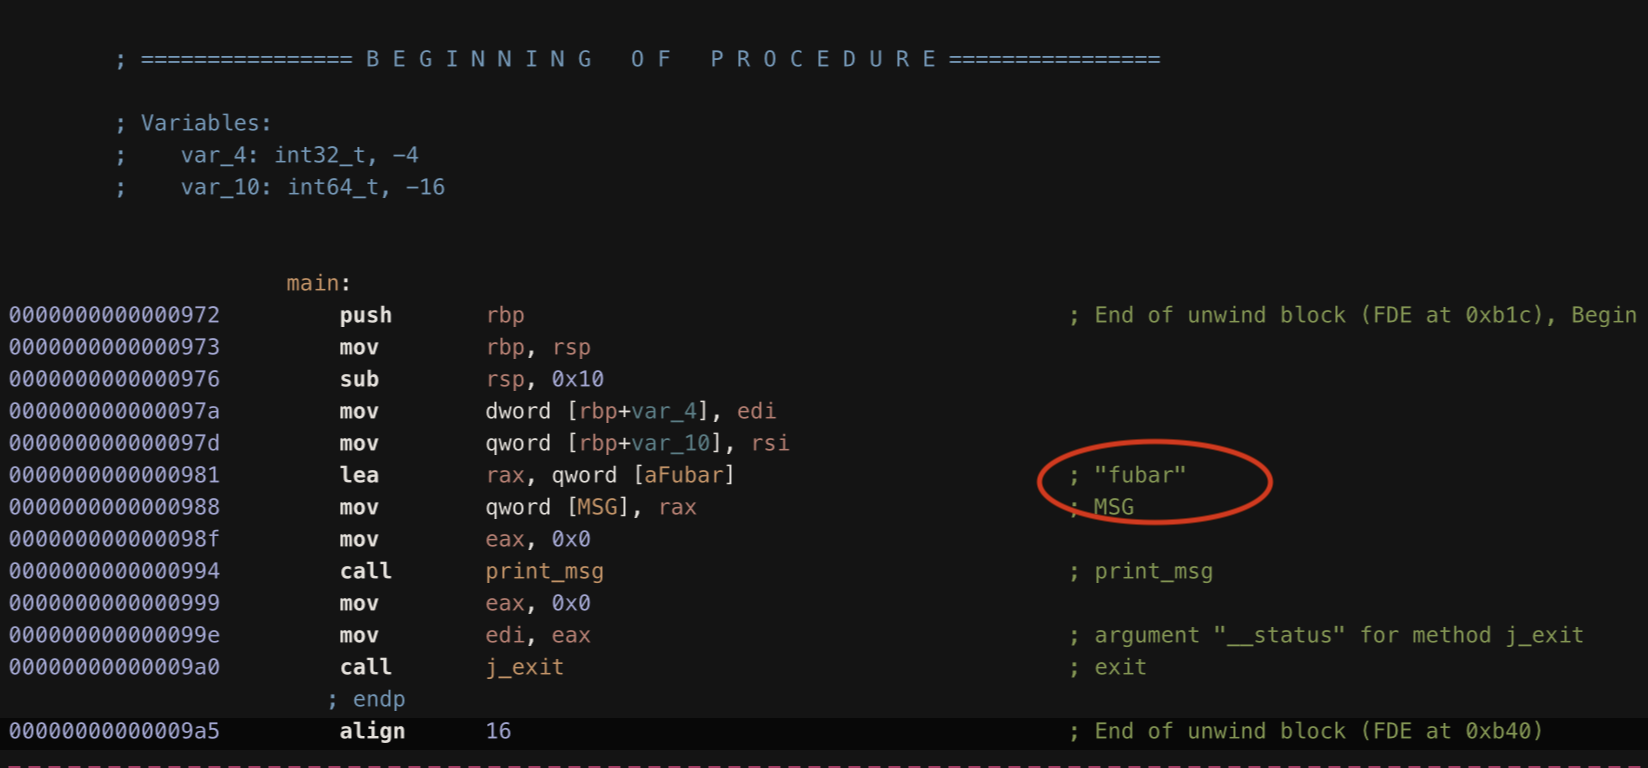
\includegraphics[width=\textwidth]{figure01.png}
%     \caption{Login Screen for Ubuntu VM.}
%     \label{fig:login}
% \end{figure}

% \begin{figure}[!ht]
%     \centering
%     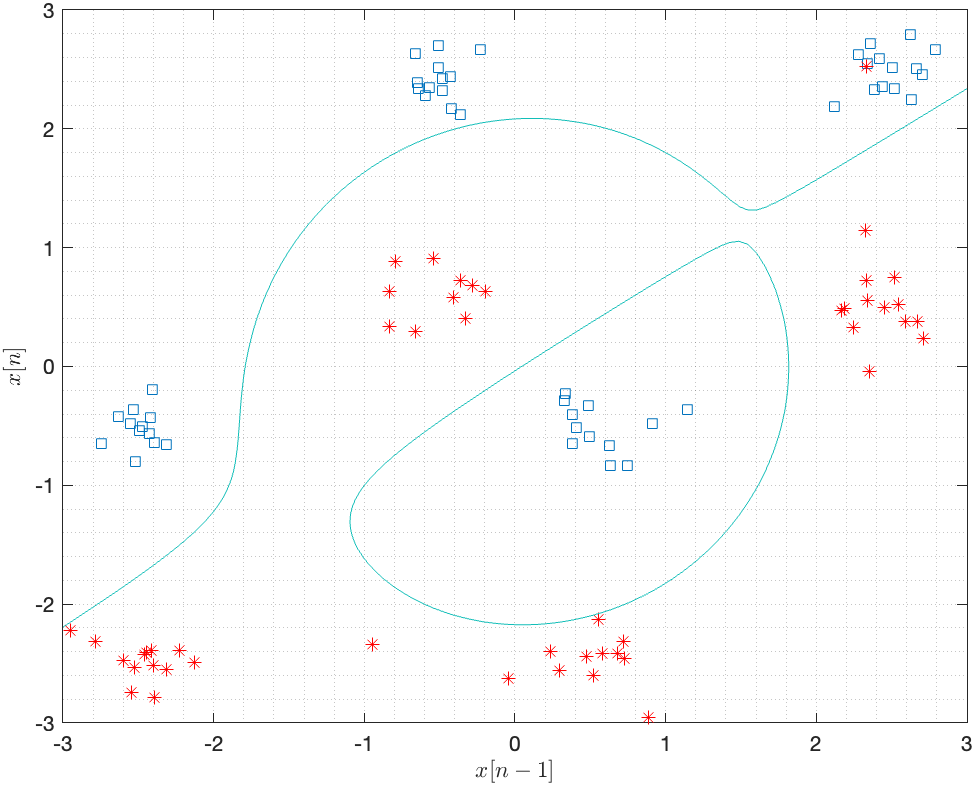
\includegraphics[width=\textwidth]{figure02.png}\vspace{-1em}
%     \caption{Settings for Ubuntu VM.}
%     \label{fig:settings}
% \end{figure}


\end{document}